\chapter{Introduction}
\say{An individual's personality is the enduring set of traits and styles that he or she exhibits, which characteristics represent (a) dispositions (i.e., natural tendencies or personal inclinations) of this person, and (b) ways in which this person differs from the \say{standard normal person} in his or her society.} \cite{personality-definition-BERGNER2020100759} This is one of the recent definitions of personality in the field of personality psychology. However, a consensus for a formal definition is yet to be established. The common aspect is that these traits and unique characteristics give both consistency and individuality to a person's behaviour. As personality is the underlying component of a person's behaviour over time and space, it is correlated to our working and social life. For example, it is reported that personality is related to job performance, job satisfaction, and productivity \cite{personality-prediction-questions-9121971}. When there is congruence between one’s personality and career, research shows that the work is engaging for the person and at the same time beneficial for the employer. Nevertheless, finding the most suitable candidates for a job description and thus extracting one's personality can be a challenging endeavour. \\

Recruiters rely on personality tests such as the Big Five personality test to supplement interviews as methods for extracting applicants. These personality questionnaires are reported to be less favored by candidates since they are time-consuming to complete \cite{personality-prediction-questions-9121971}. Therefore, interfering job-seeker's personality during an interview would save time and effort for the organization as well as the interviewees. The challenge will be to notice the connection between answers from applicants and each personality trait. A plausible solution is to monitor one's expressed emotions  which can be linked to different traits. Personality and emotions are highly related because emotion represents an integration of feeling, action, appraisal, and wants at a particular time and location while personality represents the integration over time and space of these components. A good analogy is to contemplate that \say{personality is to emotion as the climate is to weather} \cite{personality-and-emotion-revelle2009personality}. This means that what you perceive as personality, at a particular time is an emotion.  \\ 

Since the outbreak of the COVID-19 virus, there has been a paradigm shift in how people conduct their daily lives. Because multiple states enforced social distancing and issued a \say{stay at home} policy, people have made themselves even more dependent on technological tools and the web. The process of seeking jobs was also heavily affected by the pandemic since applicants were unable to meet physically for job interviews. In that regard, the interview procedure changed; going from physical meetings to video-based interviews. As a matter of fact, several corporations tend to utilize asynchronous video interviews (\acrshort{avi}s) as a part of the screening process. An AVI is an interview setting where applicants answer questions without any people from the company to be present. Here, the job-seekers reply the questions as a monologue for the recruiters to assess at a later time. The recruiters use these videos to evaluate the candidate's cognitive skills by looking at the different emotions they express when answering interview questions \cite{JOSHI20201316}. Researchers are now interested in developing systems that can assist recruiters identify emotions from candidates. This new emerging research field is called affective analytics. \\ 

Sentiment analysis, also referred to as opinion mining and emotion recognition are two types of affective analytics \cite{MSA_review2_GANDHI2023424}. In general, sentiment analysis is the computational study of people’s opinions, sentiments, emotions, appraisals, and attitudes towards entities such as products, services, organizations, individuals, issues, events, topics, and their attributes \cite{SA-definition} \cite{HP-integration-project}. Both sentiment analysis and opinion mining are considered synonyms in the literature. However, it is important to know how they are different. Papers including \cite{SA-history-MANTYLA201816} and \cite{Student-feedback-MOOCS-app11093986} describe that sentiment analysis focuses on extracting sentiment words and phrases expressing emotions, whereas opinion mining refers to finding and analyzing people's opinions towards specific entities. Emotion recognition on the other hand, is the process of recognising human emotion \cite{MSA_review2_GANDHI2023424}. According to \cite{sentiment_emotion_difference_munezero2014they}, emotion recognition can be used for identifying the polarity of sentiment when the stimulus is the entity of interest. As a result, a sentiment analysis task can be boiled down to an emotion recognition problem.\\ 

Actually, sentiment analysis is stated back to the start of human history. Research supports that extracting people's opinions has been of great interest historically: Leaders have utilized the opinions from their folk to obtain an outlook of their popularity \cite{SA-history-MANTYLA201816}. In Ancient Greece, efforts were made into detecting internal dissent. In the book \say{The Art of War}, there is a chapter called \say{Use of Spies} that concerns spy recruiting and betrayal. Political opinions were measured using voting halls from the city state of Athens in the 5th century BCE \cite{ATHEN-voting-thorley2012athenian}.  In the first decades of the twentieth century, work has been done to quantify public opinions based on several mining methods such as questionnaires, rankings, ratings, and comparisons \cite{mining-methods-droba1931methods}. Despite its historical relevance, the first academic papers on the subject were during and after WW\MakeUppercase{\romannumeral 2} where the articles were particularly politically motivated \cite{SA-history-MANTYLA201816}. What is called modern sentiment analysis had its origin in the early 2000's and the field grew rapidly in line with the World Wide Web \cite{deep-learning-WIRE}. The first academic publications focused on opinion mining from product reviews on the web \cite{describe-polarity-dave2003mining}, but sentiment analysis has expanded to multiple application domains including marketing \cite{marketing-sa-rambocas2018online}, finance \cite{stock_price1}, education \cite{education_domain}, political sciences \cite{political-science-sa-rice2021corpus}, and health care \cite{healthcare-sa-gohil2018sentiment}. \\

In recent years, there has been a shift in people's online habits; Instead of writing a customer review as a textual post on a product website, people nowadays tend to create videos and upload them to YouTube sharing their opinions about different products. Additionally, videos and images go together with user posts on other social media such as Instagram and Twitter. This transfer from a text-based to a multimodal social web has intrigued researchers to explore sentiment analysis utilizing multiple modalities (video, audio, and text), hence the name Multimodal Sentiment Analysis (\acrshort{msa}). Several recent studies have attempted to perform sentiment analysis on the social web utilizing multiple modalities. According to \cite{MSA_review1_SOLEYMANI20173}, there are currently three major lines of investment in MSA: 
%
\begin{itemize}
    \item MSA in spoken reviews and vlogs. \\
    \item MSA in human–machine and human–human interactions. \\
    \item Visual sentiment analysis analyzing images and their associated tags posted on social media.
\end{itemize}
%
\indent It is important to emphasize that MSA is not only limited to the above-mentioned lines. However, since MSA is still in its starting phase, little effort has been made into MSA for other applications such as AVIs. \\

Terms like sentiment and emotion are used interchangeably in the literature \cite{sentiment_emotion_difference_munezero2014they} \cite{HP_RPP} \cite{HP_Advanced}. They have been defined by multiple researchers from different domains. Sherer et al. \cite{scherer2005emotions} describe emotion from the perspective of cognitive appraisal theory, whereas Deonna and Teroni \cite{deonna2012emotions} define sentiment and emotion from a philosophical perspective \cite{MSA_review1_SOLEYMANI20173}. In the context of emotion recognition and sentiment analysis, emotion is a short-term disposition evoked when a person encounters a specific topic, person, or entity. Sentiment on the other hand is long-term, it is based on a longer duration.  \\

Distinguishing emotions and classifying them into categories has been widely researched, leading up to several models and theories  \cite{cross_cultural} \cite{HP_RPP} \cite{HP_Advanced}. Panksepp \cite{panksepp_book} describes the continuity of primal emotional systems in the subcortical-limbic circuits of selected areas in the mammalian brain. When stimulated these interacting systems evoke seven discrete primary emotions: seeking, anger, play, fear, care, panic-grief, and lust. The work conducted by Plutchik \cite{plutchik_model} suggests a model where emotions are based on a dimensional basis. 
%
\begin{figure}[h]
  \centering
  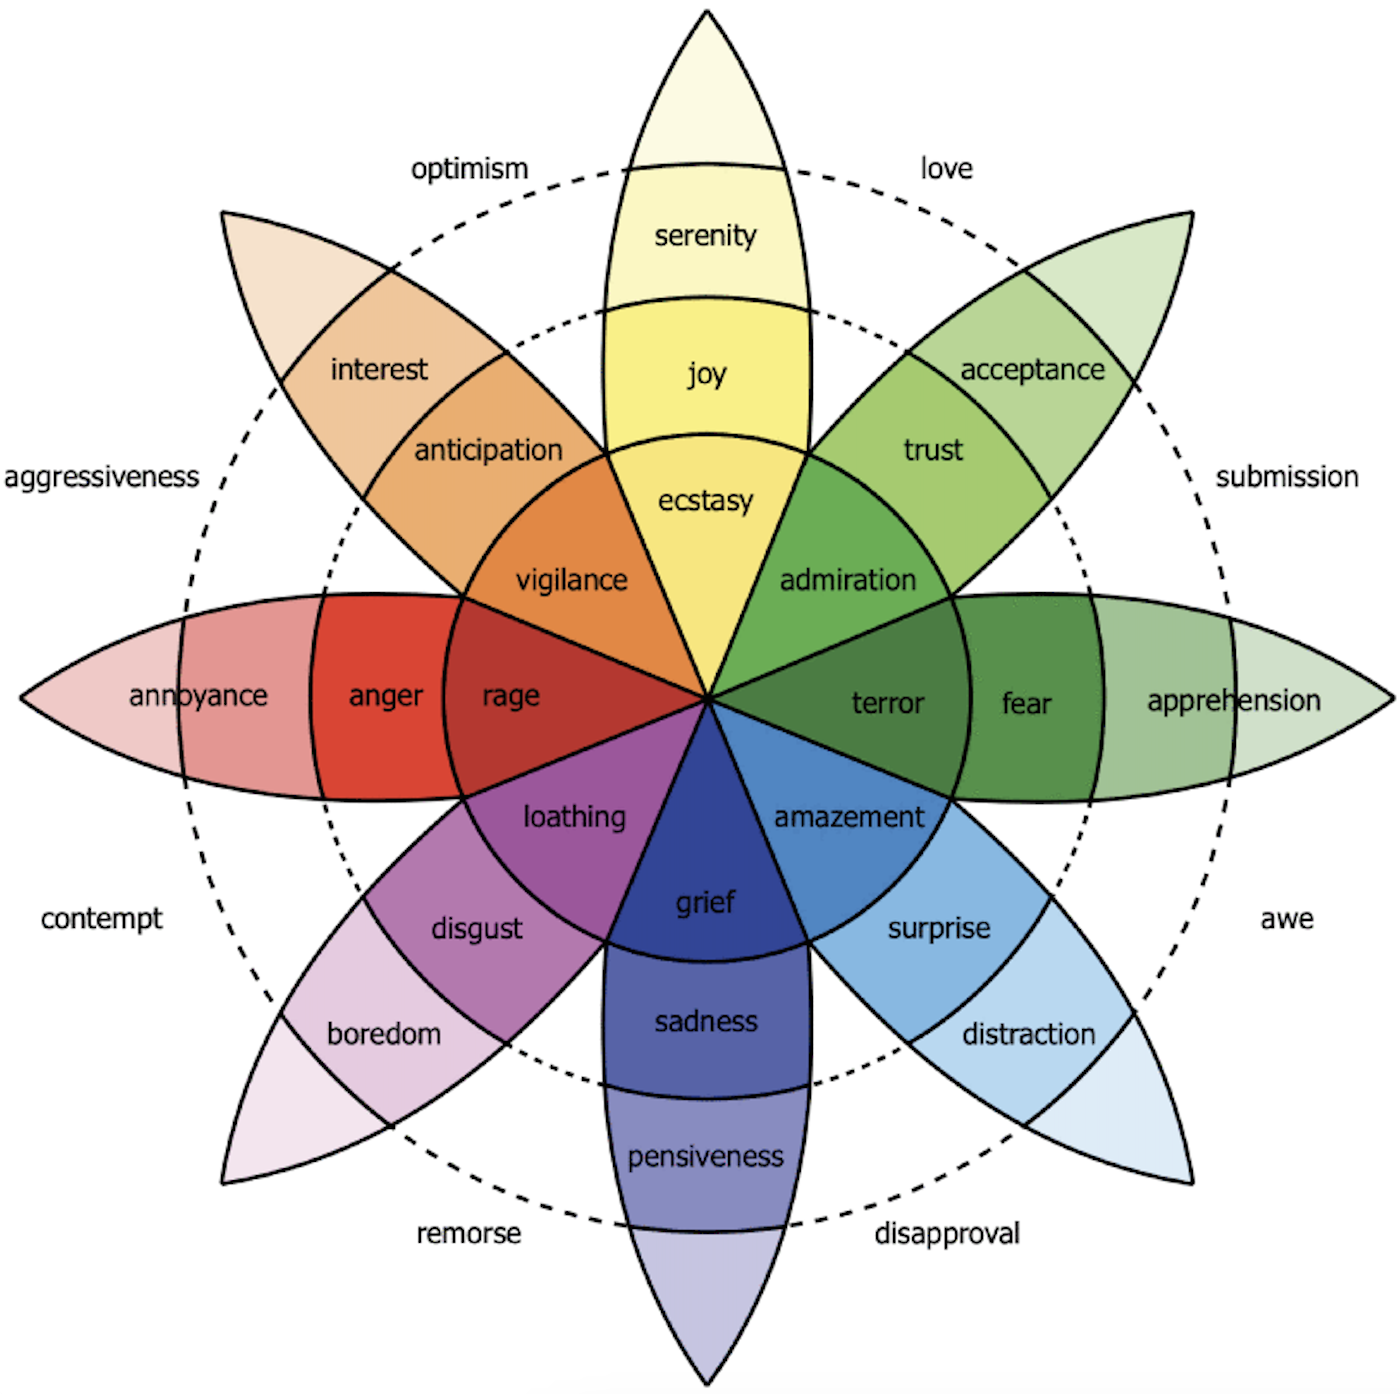
\includegraphics[width=\textwidth]{figures/plutchiks_model.png}
  \caption{Plutchik's wheel of emotions. [27]}
  \label{fig:plutchik}
\end{figure}
%
Figure \ref{fig:plutchik} depicts Plutchik's wheel of emotions which is a three-dimensional hybrid of both basic and complex categories. The eight sectors indicate that there are eight primary emotions: anger, anticipation, joy, trust, fear, surprise, sadness, and disgust. The color scheme indicates the combinations and their intensity. For example, a white color represents a mix of two emotions and a darker shade designates a more intense emotion \cite{HP_RPP} \cite{HP_Advanced}. \\

\section{Study Objective \& Research Questions}
The primary objective of this study is to understand how Artificial Intelligence (\acrshort{ai}) can be integrated into the screening process of job recruitment. The state of the questions addressed about integrating AI in recruitment reveals potentialities in emotional and personality predictions. \\

In the present investigation, the general objective is to analyze the potential of utilizing MSA in predicting the personality traits of candidates in AVIs. Throughout the study, the following research questions (RQ) will be answered:
%
\begin{itemize}
    \item[] RQ1: To what extent can MSA assist in predicting personality traits from video interviews? \\
    \item[] RQ2: Which emotions are the most relevant to predict human attributes? \\
    \item[] RQ3: What traits are most difficult to predict based on MSA in a video interview setting?  \\
    \item[] RQ4: To what extent are personality traits the same in people within the same domain? \\
\end{itemize}

\section{Contributions}
The major contributions of this Master's thesis research are as following:
\begin{itemize}
    \item Proposed an approach in prediction personality traits based on the emotion expressed in AVIs. \\
    \item Establishing a multimodal feature extraction pipeline for MSA architectures. \\
    \item Validation of detected traits via Big Five personality test. \\
    \item Providing interesting insights into assessing job applicants in today's work environment. 
\end{itemize}
%
The rest of the thesis is organized as follows: Chapter \ref{chap:background} presents the background including key concepts for the study. Related work is presented in Chapter \ref{chap:related_work}. The method is described in Chapter \ref{chap:method}, whereas results and discussion is presented in Chapter \ref{chap:results}. Lastly, Chapter \ref{chap:conclusion} concludes the thesis with potential future research directions. 
